\section{Specific Requirements} \label{sec:spec_requirements}

%More details on all aspects in Section 2 if they can be  useful for the development team

\subsection{External Interface Requirements} \label{external}

\subsubsection{User Interface} \label{user_interface}

In this section, we will present some mockup to make the reader better understand the idea of the structure of the final web page and application.

\myparagraph{Log In} 
\newline
The mockup in Figure \ref{fig:login} shows the login page of PowerEnJoy. Here, a VISITOR can log in into the application.

\vspace{70pt}

\begin{figure}[htbp]
\centering
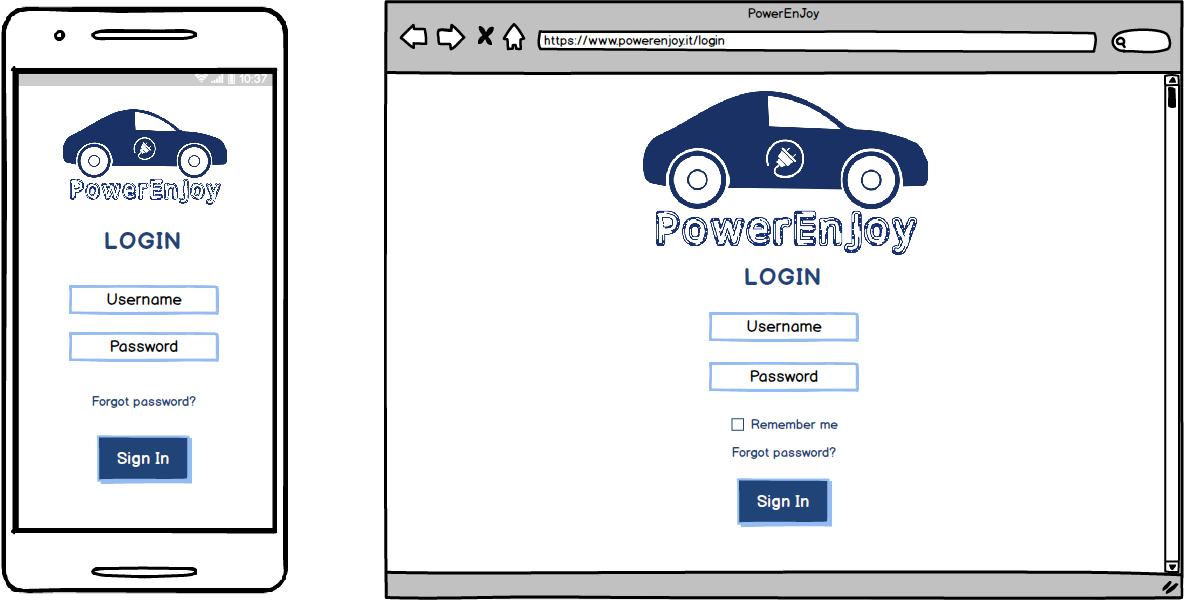
\includegraphics[width=\textwidth]{Images/Mockups/Login}
\caption{Log In Page mockup}
\label{fig:login}
\end{figure}
\clearpage

\myparagraph{Registration Form}
\newline
The mockup in Figure \ref{fig:registration} shows the registration form, where a VISITOR can sign up to access the service.

\vspace{80pt}

\begin{figure}[htbp]
\centering
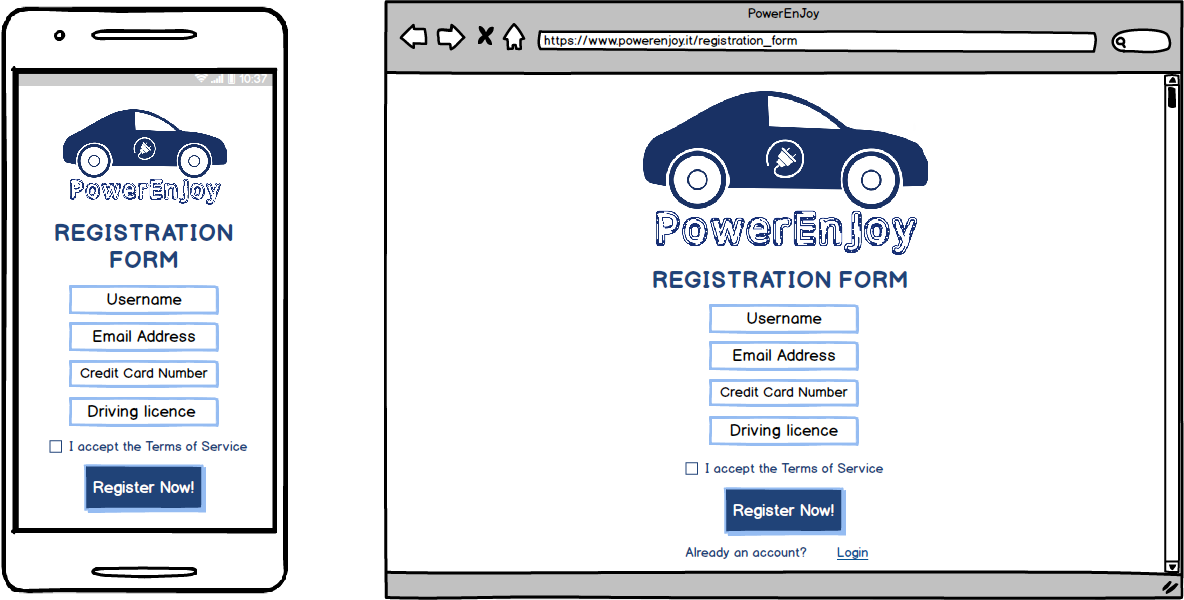
\includegraphics[width=\textwidth]{Images/Mockups/RegistrationForm}
\caption{Registration Form mockup}
\label{fig:registration}
\end{figure}
\clearpage

\myparagraph{Personal page}
\newline
The mockup in Figure \ref{fig:mypage} shows the personal page of a USER, from where he can update his data, such as, for example, the profile picture, the password and the payment information.

\vspace{80pt}

\begin{figure}[htbp]
\centering
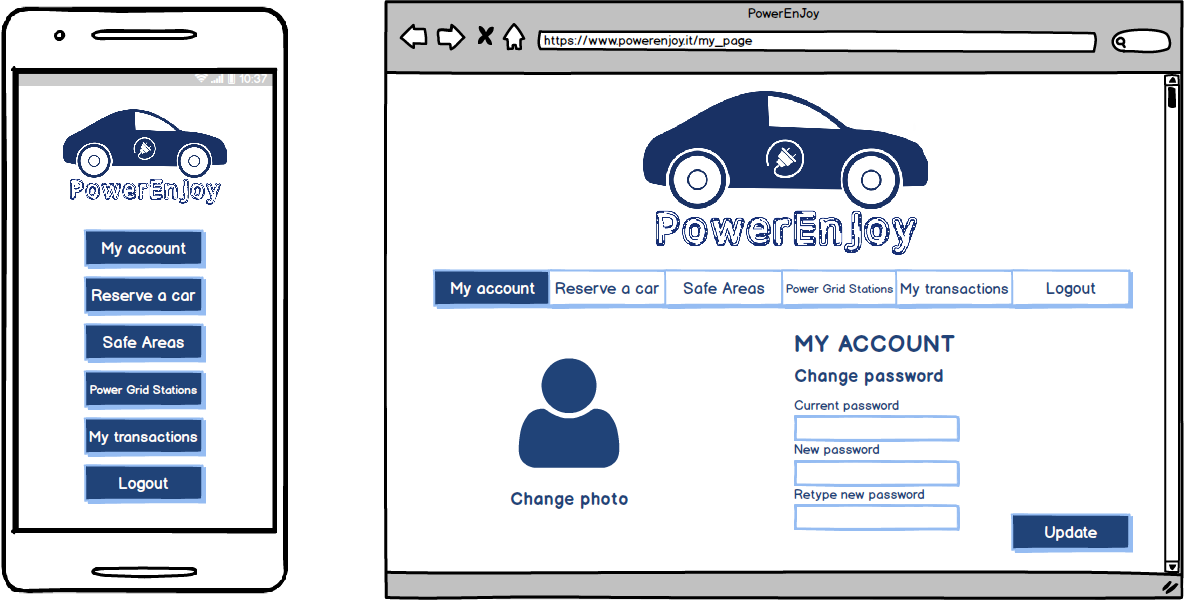
\includegraphics[width=\textwidth]{Images/Mockups/MyPage}
\caption{Personal Page mockup}
\label{fig:mypage}
\end{figure}
\clearpage

\myparagraph{Reservation page}
\newline
The mockup in Figure \ref{fig:reservation} shows the page from which a USER can reserve a car nearby him or near to a selected address for an hour.
He can also see how much time takes to get from the selected point to the car and its condition: level of charge and if it is plugged in a power grid station.

\vspace{80pt}

\begin{figure}[htbp]
\centering
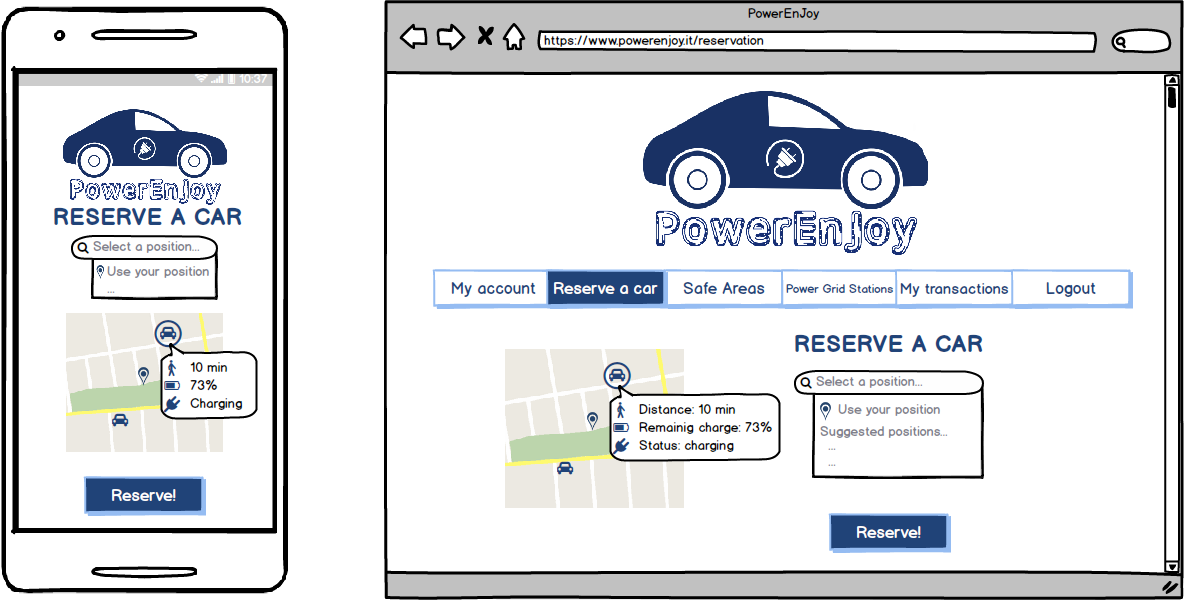
\includegraphics[width=\textwidth]{Images/Mockups/Reservation}
\caption{Reservation Page mockup}
\label{fig:reservation}
\end{figure}
\clearpage

Once the USER has made his reservation, the page and application will show him a 1 hour timer, as shown in Figure \ref{fig:timer}, in order to remind him how much time he has left to go and pick up the reserved car. In this time, the USER can decide to cancel his prenotation by clicking on the button "\textit{Cancel}". Only when the USER is nearby the car, he will be able to click the "\textit{I'm there}" button to unlock the reserved car.

\vspace{80pt}

\begin{figure}[htbp]
\centering
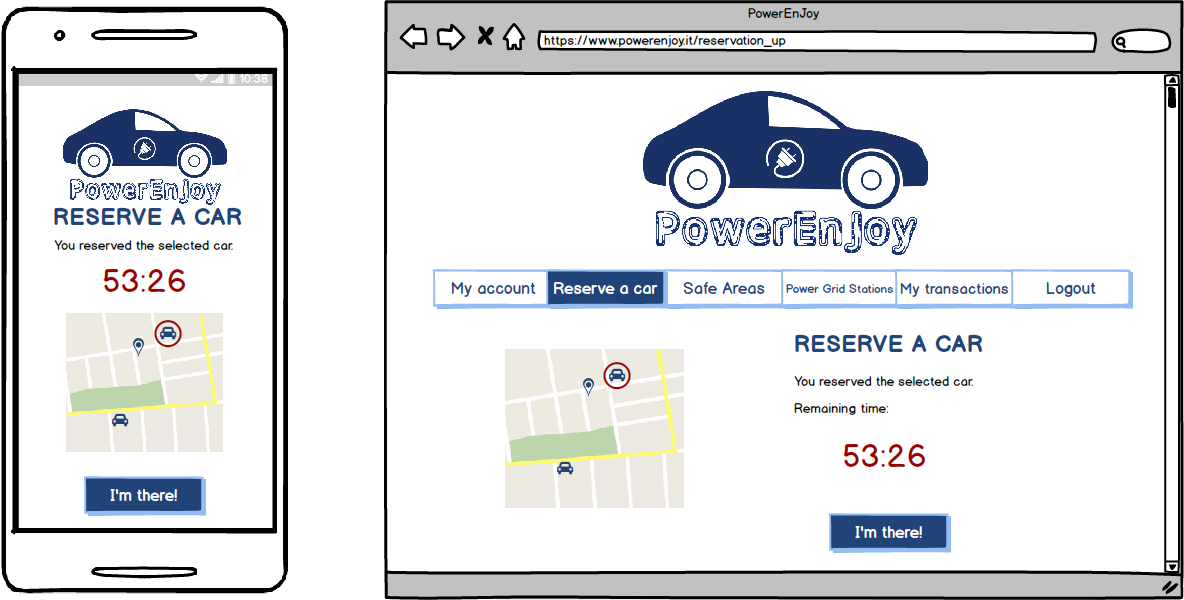
\includegraphics[width=\textwidth]{Images/Mockups/Timer}
\caption{Reservation Timer Page mockup}
\label{fig:timer}
\end{figure}
\clearpage

If the car is not picked up within an hour, the reservation expires: the USER is reminded that he has to pay a fee of 1 EUR, as shown in Figure \ref{fig:expired}.

\vspace{80pt}

\begin{figure}[htbp]
\centering
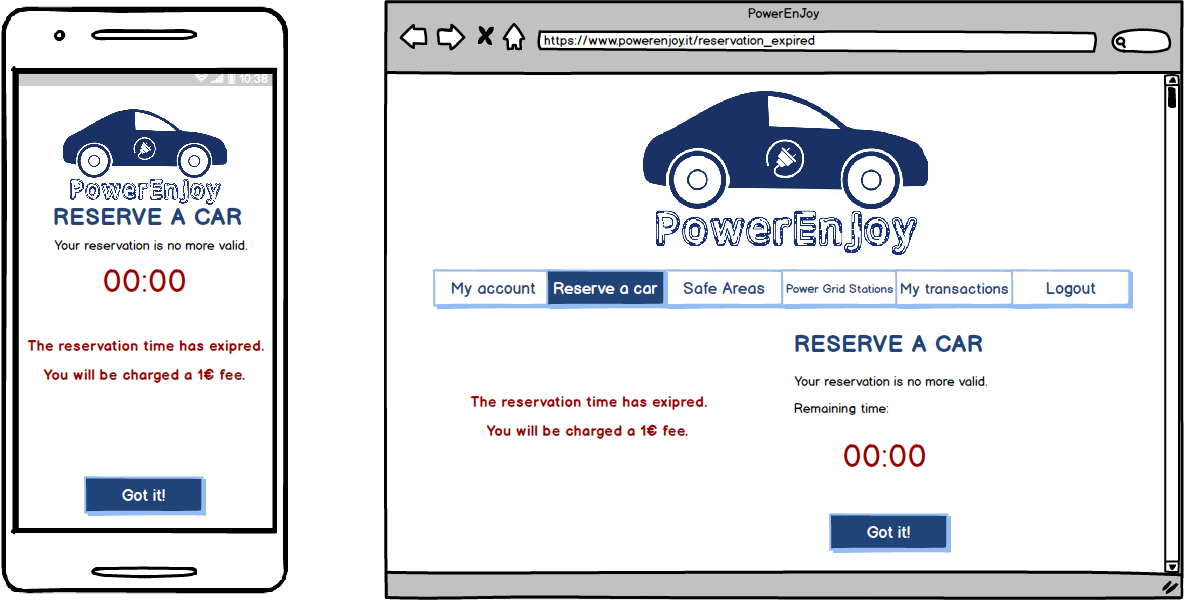
\includegraphics[width=\textwidth]{Images/Mockups/ReservationExpired}
\caption{Reservation Expired Page mockup}
\label{fig:expired}
\end{figure}
\clearpage

\myparagraph{Safe Areas page}
\newline
The mockup in Figure \ref{fig:safe} shows the page where the USER can visualize the safe areas around him or around a selected adderess.

\vspace{80pt}

\begin{figure}[htbp]
\centering
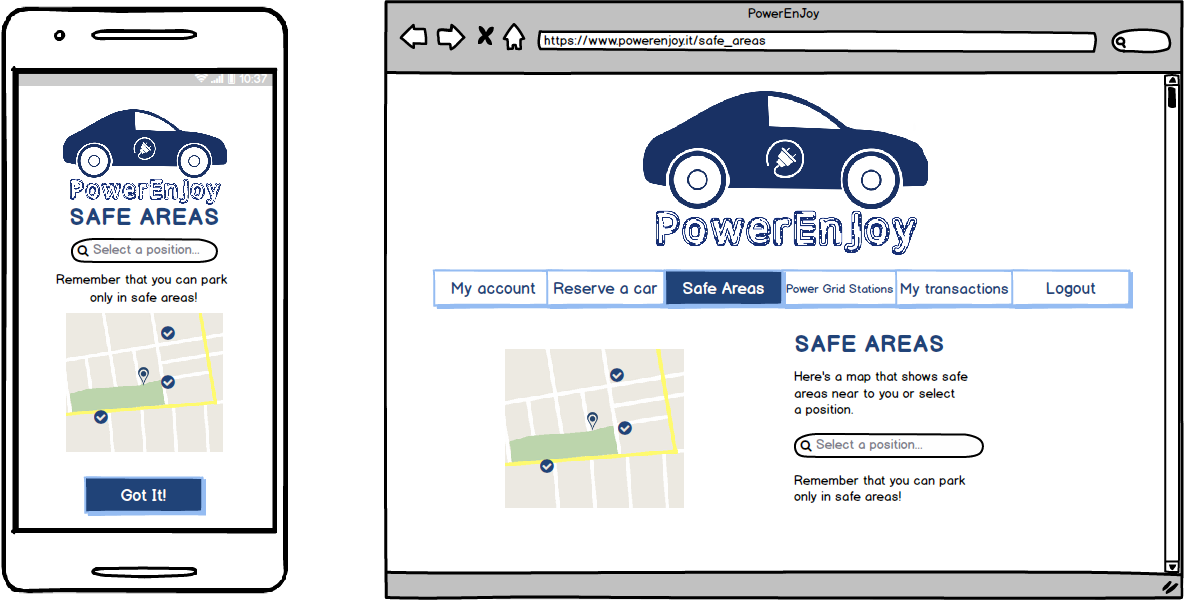
\includegraphics[width=\textwidth]{Images/Mockups/SafePlaces}
\caption{Safe Areas Page mockup}
\label{fig:safe}
\end{figure}
\clearpage

\myparagraph{Power Grid Stations page}
\newline
The mockup in Figure \ref{fig:power} shows the page where the USER can visualize the power grid stations around him or around a selected adderess.

\vspace{80pt}

\begin{figure}[htbp]
\centering
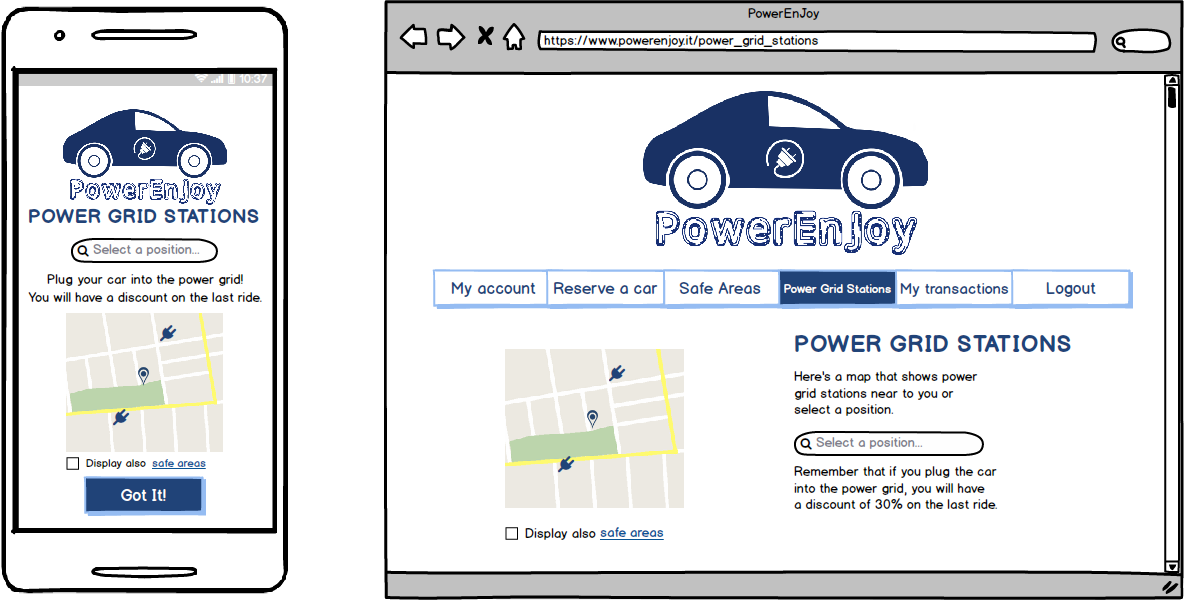
\includegraphics[width=\textwidth]{Images/Mockups/ChargePlaces}
\caption{Power Grid Station Page mockup}
\label{fig:power}
\end{figure}
\clearpage

\myparagraph{User's transactions page}
\newline
The mockup in Figure \ref{fig:transactions} shows the page where the USER can visualize his transactions and the relative details, such as the date of the ride, its duration and the discount or the increase on the fee to be payed.

\vspace{80pt}

\begin{figure}[htbp]
\centering
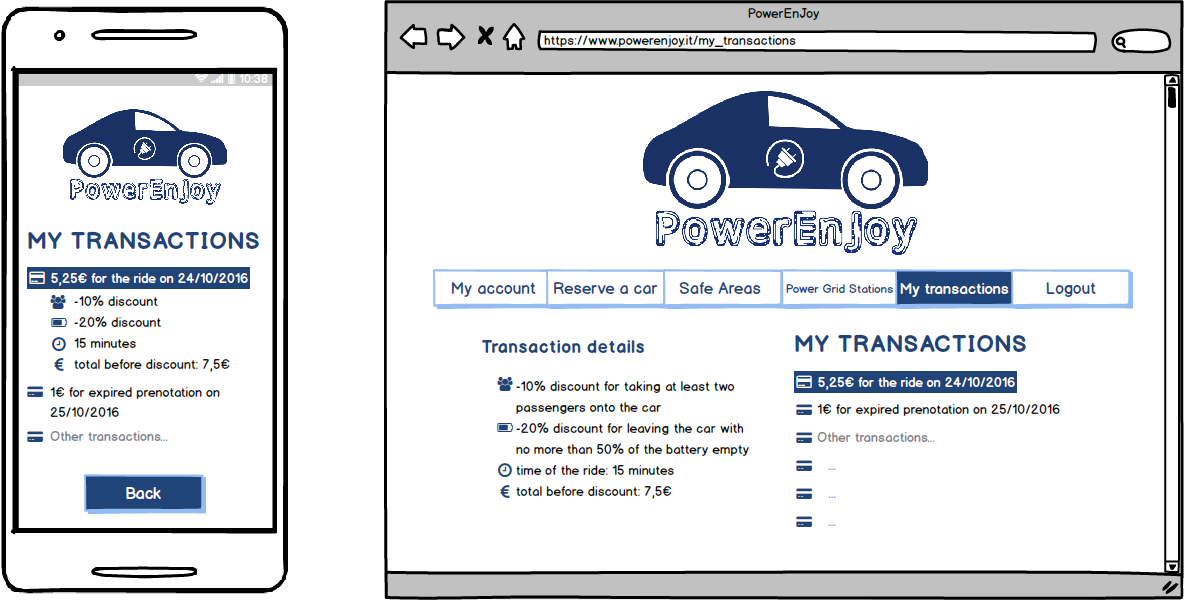
\includegraphics[width=\textwidth]{Images/Mockups/MyTransactions}
\caption{User's Transactions Page mockup}
\label{fig:transactions}
\end{figure}
\clearpage

\myparagraph{Car Screen}
\newline
The mockup in Figure \ref{fig:car} shows the car screen where useful information are visualized, for example the current level of charge, the duration of the rent and how much the USER has to pay before any discount or increase on the fee are applied.

\vspace{80pt}

\begin{figure}[htbp]
\centering
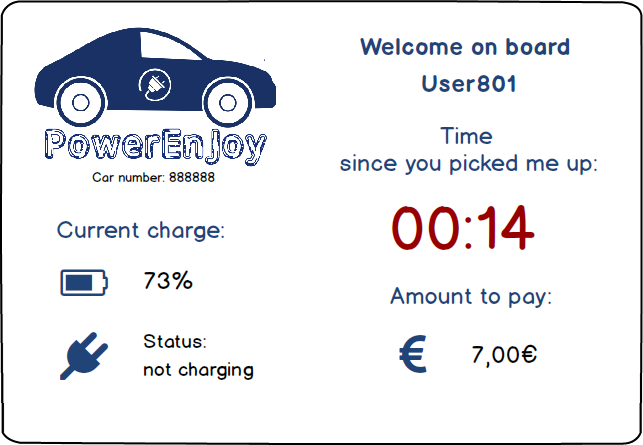
\includegraphics[width=\textwidth]{Images/Mockups/CarScreen}
\caption{Car Screen mockup}
\label{fig:car}
\end{figure}
\clearpage

\subsubsection{Hardware Interfaces} \label{hw_interfaces}
Device should be enabled with Internet and GPS receiver.

\subsubsection{Software Interfaces} \label{sw_interfaces}
The user's browser should be HTML5 compatible and the resolution should be at least 1280x720 for a satisfactory user experience.

%\subsubsection{Communication Interfaces} \label{comm_interfaces}

\subsection{Functional Requirements} \label{sec:funct_requirements}
In this section we explain all the functional requirements necessary to reach a specific goal. For each goal that was mentioned in the first section here we write its requirements.
\begin{itemize}
\item[\textbf{G1}]: 
\begin{itemize}
\item[--R1--] During the registration visitors can't choose an username already in use.
\item[--R2--] During the registration visitors can't choose an e-mail already in use.
\item[--R3--] During the registration visitors must insert valid credit card's information.
\item[--R4--] During the registration visitors must insert a valid driving license.
\item[--R5--] During the registration visitors must agree with the privacy conditions to use the system.
\end{itemize}

\item[\textbf{G2}]:
\begin{itemize}
\item[--R1--] The registration must be successfully completed.
\item[--R2--] The user must insert the correct old password.
\item[--R3--] The user must repeat twice the new password.
\item[--R4--] The user must upload a valid picture.
\end{itemize}

\item[\textbf{G3}]:
\begin{itemize}
\item[--R1--] The user must be registered at the system.
\item[--R2--] In the log in form the user must insert the correct username.
\item[--R3--] In the log in form the user must insert the correct password.
\item[--R4--] If the visitor insert the wrong data, the system shows an error and return to the log in page.
\item[--R5--] If the user doesn't remember the password he can receive it trough a special command.
\end{itemize}

\item[\textbf{G4}]:
\begin{itemize}
\item[--R1--] The user must insert a valid address or give to the system his position.
\item[--R2--] All cars position must be knowed.
\item[--R3--] All cars are set as available or not.
\item[--R4--] The list of nearest cars is made trough calculate the distance between car and user's position.
\end{itemize}

\item[\textbf{G5}]:
\begin{itemize}
\item[--R1--] The user must be correctly logged in.
\item[--R2--] The user must select which car he wants.
\item[--R3--] The user must select only date and times valid for the reservation.
\end{itemize}

\item[\textbf{G6}]:
\begin{itemize}
\item[--R1--] The position of the user and the car must be the same.
\item[--R2--] The reservation must not be expired.
\item[--R3--] The system must recognize the correct car reserved by a specific user to unlock the correct one.
\end{itemize}

\item[\textbf{G7}]:
\begin{itemize}
\item[--R1--] The car's engine must ignites.
\item[--R2--] An amount of money per minute is set.
\item[--R3--] The final charge is based on the duration of the car use.
\item[--R4--] The system must shows all user's transactions.
\item[--R5--] The user must select a specific transaction to see its details.
\end{itemize}

\item[\textbf{G8}]:
\begin{itemize}
\item[--R1--] There must be a display on the car that communicates with the system.
\item[--R2--] The charge is update every minute.
\end{itemize}

\item[\textbf{G9}]:
\begin{itemize}
\item[--R1--] It must be passed one hour from the registration.
\item[--R2--] Is applyed a fee of 1 euro to the user involved.
\item[--R3--] The reservation is deleted.
\item[--R4--] In the page there is a timer.
\end{itemize}

\item[\textbf{G10}]:
\begin{itemize}
\item[--R1--] The user must be correctly logged in.
\item[--R2--] The user must go to the reservation page.
\item[--R3--] Mustn't be passed one hour from the reservation.
\end{itemize}

\item[\textbf{G11}]:
\begin{itemize}
\item[--R1--] The reservation is correctly deleted by a user or it is expired. 
\item[--R2--] The car is set available in the list.

\end{itemize}

\item[\textbf{G12}]:
\begin{itemize}
\item[--R1--] A list of safe areas must be available to the user.
\item[--R2--] The car must be left in a safe area.
\item[--R3--] The user and all any passengers must exit from the car.
\end{itemize}

\item[\textbf{G13}]:
\begin{itemize}
\item[--R1--] The car must be used by a user.
\item[--R2--] Discounts are in a list where is defined all details.
\item[--R3--] In the car there is a sensor which counts how many people there are in the car, if they are three or more a discount is applied.
\item[--R4--] In the car there is a sensor which controls how many battery is empty, if it is no more than 50 per cent the system applied a discount.
\item[--R5--] If the user takes care to link the car to recharge the car he will have a discount.
\end{itemize}

\item[\textbf{G14}]:
\begin{itemize}
\item[--R1--] The car must have been recently used.
\item[--R2--] Most of 80 per cent of the battery is empty.
\item[--R3--] The car is left far away from a safe area.
\end{itemize}


\item[\textbf{G15}]:
\begin{itemize}
\item[--R1--] The user must go to the specific page.
\item[--R2--] The user must insert a correct position. 
\end{itemize}


\item[\textbf{G16}]:
\begin{itemize}
\item[--R1--] The user must go to the specific page.
\item[--R2--] The user must insert a correct position.
\end{itemize}
\end{itemize}

\subsection{Scenario Identification} \label{sec:scenarios}
\subsubsection{Scenario 1: Registration and Log in} \label{sce1}
Monica is a ecologist girl who everyday goes at work by train because her work place is attainable only by train or by car. One day she goes to the train station but there is a strike, she is desperate: how can she go to work? Talking with other people in the station she learns that exists a car-sharing that provides only electric cars and that she can reserve a car trough an application on her mobile phone, this application is "\textit{PowerEnJoy}". She quickly goes to the web site and download the app but to use it she must register giving some data, her driving license number and her credit card information; she insert all the correct data and as soon as she press the registration button in her mail box arrives a new e-mail with a password to access the system: she is now a new user. In the log in page she insert her username and the password recieved so she can easily enter in the system. Monica is now in her personal page where she can change the password or insert a picture to personalize her profile.
\subsubsection{Scenario 2: Reserve a car} \label{sce2}
Mario wants to reserve an electric car to go with his girlfriend to have a pic-nic in a beautiful meadow in mountain. He quickly enters in the "\textit{PowerEnJoy}" app and goes to the reservation page that is very simple to use: he only must insert a position and the system will search for an available car nearby. In the box he can insert his specific position activating his Smartphone GPS or insert a different one: he chooses the first option. In the map on the reservation page appear immediately two cars that are available, when he select one of them he can see a curtain with the time distance between him and the car, the car's level of the battery and its status like "charging". He choose the best one and pressed the button "\textbf{\textit{Reserve!}}": immediately the reservation is confirmed and appears a timer to remind him that he has one hour to pick up the car.
\subsubsection{Scenario 3: Pick up a car} \label{sce3}
Luca has reserved a car and now, thanks to the map in the reservation page, he walked towards the car. As soon as he is nearby the car he pressed the button "\textbf{\textit{I'm there!}}", the system compares his position and the car's position: they are the same so the car is unlocked and Luca can enter in it. In the car there is a screen where he can see his username, the car's number, the battery level so he can know when he must charge the car and, very important, the time passed from the moment he has picked up the car with the corresponding amount to pay.
\subsubsection{Scenario 4: Charge, park and lock a car} \label{sce4}
Maria is, from a long time, using a car picked up through the "\textit{PowerEnJoy}" app, she goes everywhere to do shopping so she consume a lot of battery. She see that the battery level is low and she must charge it; she know that in the app there is a page to consult the list of power grid station near a specific position so no one will remain "on foot". She access the app using her Smartphone and goes to the needed page, she activates her GPS so in the map appears a station that she can reach quickly; when she arrives she links the car to charge it. After that she continues her shopping; when she has finished all the commissions she wants to park the car in a safe area so, just as she has done before, she goes to the safe area's page, insert her position and a list of areas will appears on the map. She chooses for the best one and goes there, as soon as she park the car and exit from it the system automatically lock it.  
\subsubsection{Scenario 5: Transaction} \label{sce5}
Fabio is in a shop and, at the moment to pay, the shop assistant tell to him that he has reached the daily credit card's limit. He is furious and can not understand how it is possible, suddenly he reminds that in the morning he has picked up a car from "\textit{PowerEnJoy}" and he thinks that the system has charged him more than necessary. Fortunately in the app there is a page with the details of all the transaction; he access in his personal page and goes to the transaction's page: here there is a list and, when one of the list entry is selected, all its details appear. He selected that corresponding to the morning reservation: the charge is correct because is specified the time of car using and the amount calculates from a specified cost per minute. He has spent his money in an another way.
\subsubsection{Scenario 6: Reservation expired} \label{sce6}
Giusy telephone starts ringing: is her best friend who tells that she not need to share a car because someone will go to get her. Giusy has already make a car reservation but she knows that she can delete it without problems because in the app reservation page there is a button specific to do this action. "There is no hurry" thinks Giusy so she continues to do her work: she has forget that the reservation will last only one hour. After a lot of time she remember that has not delete the car reservation yet so she takes her computer and goes to the site but when she arrives at the reservation's page there is a surprise: the timer strikes 00:00 and there is a red written " The reservation time is expired. You will be charged 1 euro fee.". Next time she will pay more attention. 
\clearpage  

\subsection{UML Models}
\subsubsection{Use Case Diagram}

The Figure \ref{fig:use case} shows the actors involved in the system, how they relate with it and all the ways in which they can use the functionalities provided by "\textit{PowerEnJoy}".  


\begin{figure}[htbp]
\centering
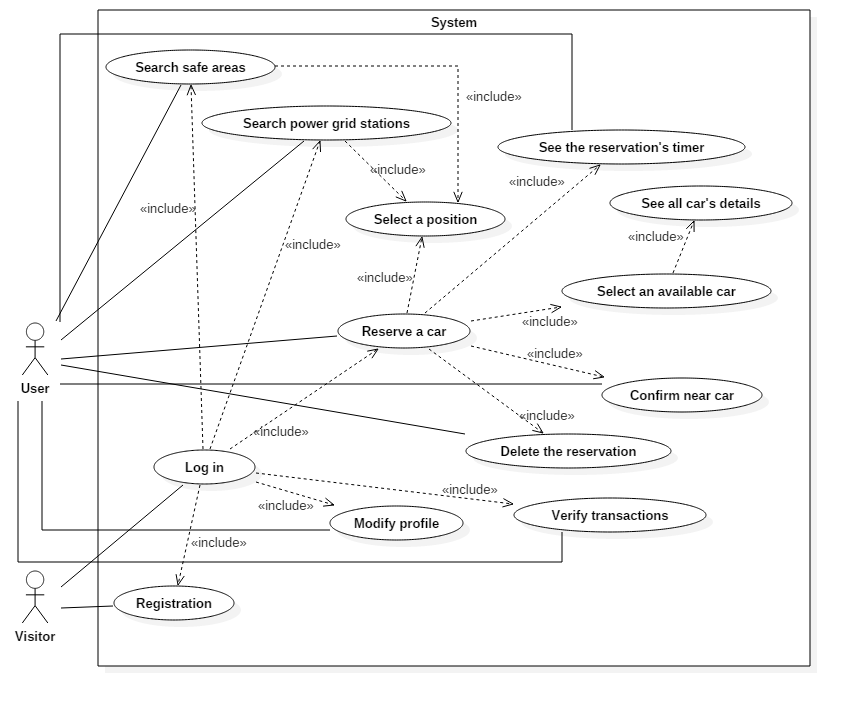
\includegraphics[width=\textwidth]{Images/UML/UseCase}
\caption{Use Case Diagram}
\label{fig:use case}
\end{figure}
\clearpage

\subsubsection{Use Case Description}
\myparagraph{Registration}
\newline
\begin{table}[htb]
\begin{center}
\renewcommand{\arraystretch}{1.5}
\begin{tabular}{|l|p{0.6\textwidth}|}
\hline
Actor & Visitor \\ \hline
Goal & \textbf{G1} \\ \hline
Requirements Associated & G1.\textbf{R1},G1.\textbf{R2},G1.\textbf{R3},G1.\textbf{R4},G1.\textbf{R5} \\ \hline
Precondition & The Visitor reach the registration form after access the application home page \\ \hline
Trigger & The Visitor has press the "Register Now!" button \\ \hline
Successful end condition & The Visitor is now a new User \\ \hline
Failed end condition & The Visitor is requested to try again because an error occurs \\ \hline
Main flow & \begin{minipage}[t]{0.6\textwidth}
\begin{enumerate}
\addtolength{\itemindent}{0.5cm}
\item The Visitor completes the registration form with all the necessary data.
\item The Visitor submits the form.
\item The system verifies that nickname and e-mail are not in used.
\item The system saves all the visitor's data in the database.
\item The system shows a confirmation message.
\end{enumerate}
\end{minipage} \\ \hline
Extensions & \\ \hline
Inclusions & "See the registration form" \\ \hline
\end{tabular}
\caption{Registration Use Case}
\end{center}
\end{table}
\clearpage

\myparagraph{Log In}
\newline
\begin{table}[htb]
\begin{center}
\renewcommand{\arraystretch}{1.5}
\begin{tabular}{|l|p{0.6\textwidth}|}
\hline
Actor & Visitor \\ \hline
Goal & \textbf{G3} \\ \hline
Requirements Associated & G3.\textbf{R1},G3.\textbf{R2},G3.\textbf{R3},G3.\textbf{R4},G3.\textbf{R5} \\ \hline
Precondition & The Visitor reach the log in form after correctly register at the system \\ \hline
Trigger & The Visitor has press the "Sign In!" button \\ \hline
Successful end condition & The Visitor is now a User and can do all the operations \\ \hline
Failed end condition & The Visitor doesn't insert the correct data or is not registered \\ \hline
Main flow & \begin{minipage}[t]{0.6\textwidth}
\begin{enumerate}
\addtolength{\itemindent}{0.5cm}
\item The Visitor insert username and password.
\item The Visitor submits the log in form.
\item The system verifies the data.
\item The system shows the User page.
\end{enumerate}
\end{minipage} \\ \hline
Extensions & \\ \hline
Inclusions & "Registration","Modify profile", "Verify transactions", "Reserve a car", "Search power grid stations", "Search safe areas"  \\ \hline
\end{tabular}
\caption{Log in Use Case}
\end{center}
\end{table}
\clearpage

\myparagraph{Modify profile}
\newline
\begin{table}[htb]
\begin{center}
\renewcommand{\arraystretch}{1.5}
\begin{tabular}{|l|p{0.6\textwidth}|}
\hline
Actor & User \\ \hline
Goal & \textbf{G2} \\ \hline
Requirements Associated & G2.\textbf{R1},G2.\textbf{R2},G2.\textbf{R3},G2.\textbf{R4} \\ \hline
Precondition & The User must be logged in \\ \hline
Trigger & The User has press the "Update" button \\ \hline
Successful end condition & The User's data are correctly upadated \\ \hline
Failed end condition & The new data are not correctly updated \\ \hline
Main flow & \begin{minipage}[t]{0.6\textwidth}
\begin{enumerate}
\addtolength{\itemindent}{0.5cm}
\item The Visitor insert old password and/or a new picture.
\item The Visitor submits the update form.
\item The system verifies the data.
\item The system must save the new update in the database.
\item The system shows a confirmation message.
\end{enumerate}
\end{minipage} \\ \hline
Extensions & \\ \hline
Inclusions &  \\ \hline
\end{tabular}
\caption{Modify profile Use Case}
\end{center}
\end{table}
\clearpage

\myparagraph{Verify transactions}
\newline
\begin{table}[htb]
\begin{center}
\renewcommand{\arraystretch}{1.5}
\begin{tabular}{|l|p{0.6\textwidth}|}
\hline
Actor & User \\ \hline
Goal & \textbf{G7} \\ \hline
Requirements Associated & G7.\textbf{R4},G7.\textbf{R5} \\ \hline
Precondition & The User must be logged in \\ \hline
Trigger & The User has selected a specific transaction from a list \\ \hline
Successful end condition & The User see all the selected transaction's details \\ \hline
Failed end condition & The User receives an error message \\ \hline
Main flow & \begin{minipage}[t]{0.6\textwidth}
\begin{enumerate}
\addtolength{\itemindent}{0.5cm}
\item The system shows all the user's transaction.
\item The User selects one form the list.
\end{enumerate}
\end{minipage} \\ \hline
Extensions & \\ \hline
Inclusions &  \\ \hline
\end{tabular}
\caption{Verify transaction Use Case}
\end{center}
\end{table}
\clearpage

\myparagraph{Search safe area}
\newline
\begin{table}[htb]
\begin{center}
\renewcommand{\arraystretch}{1.5}
\begin{tabular}{|l|p{0.6\textwidth}|}
\hline
Actor & User \\ \hline
Goal & \textbf{G15} \\ \hline
Requirements Associated & G15.\textbf{R1},G15.\textbf{R2} \\ \hline
Precondition & The User must be logged in \\ \hline
Trigger & The User has insert a correct position. \\ \hline
Successful end condition & The User see all the nearest safe areas \\ \hline
Failed end condition & The User receives an error message \\ \hline
Main flow & \begin{minipage}[t]{0.6\textwidth}
\begin{enumerate}
\addtolength{\itemindent}{0.5cm}
\item The user insert a correct position or activate the GPS.
\item The system shows on the map the safe areas.
\item The system must have a list of all the safe areas.
\end{enumerate}
\end{minipage} \\ \hline
Extensions & \\ \hline
Inclusions & "Select a position" \\ \hline
\end{tabular}
\caption{Search safe area Use Case}
\end{center}
\end{table}
\clearpage

\myparagraph{Search power grid station}
\newline
\begin{table}[htb]
\begin{center}
\renewcommand{\arraystretch}{1.5}
\begin{tabular}{|l|p{0.6\textwidth}|}
\hline
Actor & User \\ \hline
Goal & \textbf{G16} \\ \hline
Requirements Associated & G16.\textbf{R1},G16.\textbf{R2} \\ \hline
Precondition & The User must be logged in \\ \hline
Trigger & The User has insert a correct position. \\ \hline
Successful end condition & The User see all the nearest power grid stations \\ \hline
Failed end condition & The User receives an error message \\ \hline
Main flow & \begin{minipage}[t]{0.6\textwidth}
\begin{enumerate}
\addtolength{\itemindent}{0.5cm}
\item The user insert a correct position or activate the GPS.
\item The system shows on the map the power grid stations.
\item The system must have a list of all the power grid stations.
\end{enumerate}
\end{minipage} \\ \hline
Extensions & \\ \hline
Inclusions & "Select a position" \\ \hline
\end{tabular}
\caption{Search power grid station Use Case}
\end{center}
\end{table}
\clearpage

\myparagraph{Reserve a car}
\newline
\begin{table}[htb]
\begin{center}
\renewcommand{\arraystretch}{1.5}
\begin{tabular}{|l|p{0.6\textwidth}|}
\hline
Actor & User \\ \hline
Goal & \textbf{G4},\textbf{G5} \\ \hline
Requirements Associated & G4.\textbf{R1},G4.\textbf{R2},G4.\textbf{R3},G4.\textbf{R4}, G5.\textbf{R1},G5.\textbf{R2},G5.\textbf{R3} \\ \hline
Precondition & The User must be logged in \\ \hline
Trigger & The User has pressed the "Reserve!" button \\ \hline
Successful end condition & The User see all the nearest available cars \\ \hline
Failed end condition & The User receives an error message \\ \hline
Main flow & \begin{minipage}[t]{0.6\textwidth}
\begin{enumerate}
\addtolength{\itemindent}{0.5cm}
\item The user insert a correct position or activate the GPS.
\item The system shows on the map the available car.
\item The User must select one of the cars.
\item The system must shows all the selected car's detail.
\item The User must submit the reservation form.
\item The system saves all the reservation's details and start shows a timer. 
\end{enumerate}
\end{minipage} \\ \hline
Extensions & \\ \hline
Inclusions & "Select a position","Delete the reservation", "Confirm near car", "Select an available car"( that includes "See all car's details"), "See the reservation's timer" \\ \hline
\end{tabular}
\caption{Reserve a car Use Case}
\end{center}
\end{table}
\clearpage

\myparagraph{Delete a reservation}
\newline
\begin{table}[htb]
\begin{center}
\renewcommand{\arraystretch}{1.5}
\begin{tabular}{|l|p{0.6\textwidth}|}
\hline
Actor & User \\ \hline
Goal & \textbf{G10},\textbf{G11} \\ \hline
Requirements Associated & G10.\textbf{R1},G10.\textbf{R2},G10.\textbf{R3},G11.\textbf{R1},G11.\textbf{R2} \\ \hline
Precondition & The User must have made a reservation \\ \hline
Trigger & The User has pressed the "Delete!" button \\ \hline
Successful end condition & The User receives a confirmation message \\ \hline
Failed end condition & The User receives an error message \\ \hline
Main flow & \begin{minipage}[t]{0.6\textwidth}
\begin{enumerate}
\addtolength{\itemindent}{0.5cm}
\item The user go to the reservation page.
\item The reservation must not be expired.
\item The system must set the car as available. 
\end{enumerate}
\end{minipage} \\ \hline
Extensions & \\ \hline
Inclusions & \\ \hline
\end{tabular}
\caption{Delete a reservation Use Case}
\end{center}
\end{table}
\clearpage

\myparagraph{Confirm to be near the reserved car}
\newline
\begin{table}[htb]
\begin{center}
\renewcommand{\arraystretch}{1.5}
\begin{tabular}{|l|p{0.6\textwidth}|}
\hline
Actor & User \\ \hline
Goal & \textbf{G6} \\ \hline
Requirements Associated & G6.\textbf{R1},G6.\textbf{R2},G6.\textbf{R3} \\ \hline
Precondition & The User must have made a reservation and must be near the car \\ \hline
Trigger & The User has pressed the "I'm There!" button \\ \hline
Successful end condition & The car in unlocked \\ \hline
Failed end condition & The car remains locked \\ \hline
Main flow & \begin{minipage}[t]{0.6\textwidth}
\begin{enumerate}
\addtolength{\itemindent}{0.5cm}
\item The user go to the reservation page.
\item The reservation must not be expired.
\item The position of the user and the car must be the same. 
\end{enumerate}
\end{minipage} \\ \hline
Extensions & \\ \hline
Inclusions & \\ \hline
\end{tabular}
\caption{ Confirm to be near the reserved car Use Case}
\end{center}
\end{table}
\clearpage

\myparagraph{See the reservation timer}
\newline
\begin{table}[htb]
\begin{center}
\renewcommand{\arraystretch}{1.5}
\begin{tabular}{|l|p{0.6\textwidth}|}
\hline
Actor & User \\ \hline
Goal & \textbf{G9} \\ \hline
Requirements Associated & G9.\textbf{R4} \\ \hline
Precondition & The User must have made a reservation \\ \hline
Trigger & The User goes to the reservation page \\ \hline
Successful end condition & The timer is showed \\ \hline
Failed end condition & The User receives an error message \\ \hline
Main flow & \begin{minipage}[t]{0.6\textwidth}
\begin{enumerate}
\addtolength{\itemindent}{0.5cm}
\item The user go to the reservation page.
\item The user must have made a reservation. 
\end{enumerate}
\end{minipage} \\ \hline
Extensions & \\ \hline
Inclusions & \\ \hline
\end{tabular}
\caption{ See the reservation timer Use Case}
\end{center}
\end{table}
\clearpage


\subsection{Performance Requirements} \label{sec:perf_requirements}
Performance must be acceptable to garantee a quiet good level of usability, in fact we supposed the time between the reservation confirmation and the timer start is equal to zero as well as the time between the user arrival near the car and its unlock. The system performance is closely linked with user internet connection and so indipendent from our develop.

\subsection{Design Constraints} \label{sec:design_constr}
All design constraints are linked with the language used to program.

\subsection{Software System Attributes} \label{sec:sw_sys_attr}
\subsubsection{Availability} \label{availability}
Our system can be accessed in each time the user wants, it's only needs the internet connection so its availability is closely related to it presence. The fact that the system is always accessible does not guarantee the presence of available car: this is indipendent from our system.

\subsubsection{Security} \label{security}
The user's data are all protected by the use of password and database's cryptography trough MD5 function. The transaction must be authorized by the user's bank and all its details are consultable in a user's page called "\textit{My Transaction}" so the user can be sure that his credit card will not be used illegally.

\subsubsection{Maintainability} \label{maintainability}
The system maintainability depends on the API's develop but thanks to all the document it will be simple in the future to adapt the software to any change.

\subsubsection{Portability} \label{portability}
The application can be used to any \acs{os} so it has a very good portability.

\subsection{Other Requirements} \label{other}
